% Which Open Problems Might Remain Beyond LLM-Based Systems?  (Armand Rochette, 2026)
% Self-contained LaTeX source. Compile twice with pdflatex (TeX Live 2023 or later).
% Packages used: mathpazo, helvet, courier, tikz, pgfplots, booktabs, tabularx, longtable, xurl, hyperref.
\documentclass[11pt,a4paper]{article}
\usepackage[T1]{fontenc}
\usepackage[utf8]{inputenc}
\usepackage{mathpazo}
\usepackage[scaled=0.92]{helvet}
\usepackage{courier}
\linespread{1.04}
\usepackage[a4paper,margin=2.4cm]{geometry}
\usepackage{amsmath,amssymb,amsthm}
\usepackage{booktabs,tabularx,array,longtable}
\usepackage{graphicx}
\usepackage[dvipsnames]{xcolor}
\usepackage{tikz}
\usetikzlibrary{positioning,arrows.meta,shapes.geometric,calc}
\usepackage{pgfplots}
\pgfplotsset{compat=1.18}
\usepackage{enumitem}
\usepackage[font=small,labelfont=bf]{caption}
\usepackage{microtype}
\usepackage{xurl}
\usepackage{float}
\usepackage{placeins}
\renewcommand{\arraystretch}{1.18}
\usepackage[colorlinks=true,linkcolor=MidnightBlue,citecolor=MidnightBlue,urlcolor=MidnightBlue,pdftitle={Which Open Problems Might Remain Beyond LLM-Based Systems?},pdfauthor={Armand Rochette},pdfsubject={A falsification-driven search for criteria and candidate problems},pdfkeywords={large language models, open problems, falsification, mathematics}]{hyperref}

\urlstyle{same}
\newtheoremstyle{prob}{8pt}{8pt}{\normalfont}{}{\bfseries}{.}{0.5em}{}
\theoremstyle{prob}
\newtheorem{problem}{Problem}
\newcolumntype{L}[1]{>{\raggedright\arraybackslash}p{#1}}
\newcolumntype{Y}{>{\raggedright\arraybackslash}X}
\setlist{itemsep=2pt,topsep=4pt}
\setlength{\intextsep}{10pt plus 2pt minus 2pt}
\setlength{\textfloatsep}{12pt plus 2pt minus 2pt}
\newcommand{\Cone}{\textbf{C1}}
\newcommand{\Ctwo}{\textbf{C2}}

\title{\textbf{Which Open Problems Might Remain Beyond LLM-Based Systems?}\\[6pt]
\large A falsification-driven search for criteria and candidate problems}
\author{Armand Rochette\thanks{The author can be contacted through the issue tracker of the repository \url{https://github.com/tbop/open-problems-beyond-llm-reach}. The use of AI in this work is described in the AI disclosure at the end of the paper. The document has not been peer reviewed.}}
\date{22 November 2026}

\begin{document}
\maketitle

\begin{abstract}
\noindent In 2026, systems built on large language models (LLMs) have been reported to resolve hundreds of open mathematical problems. We ask whether one can state criteria, derived from how such systems work, that single out problems they are unlikely to solve. We proceeded by falsification: a set of criteria is rejected as soon as one problem meets all of them and has nevertheless been reported solved by AI. Six versions of the criteria were tested against a corpus consisting of the 373 result families of OpenAI's October 2026 mathematics release and ten further reported results, among them the claimed proofs of the Riemann Hypothesis and of Navier--Stokes blow-up. Architectural arguments did not survive the move from a bare model to a full system with tools, and criteria based on novelty did not survive the evidence. The surviving set has two criteria on top of a scope condition: the problem is \emph{prominent}, and it has \emph{no non-trivial partial result in either direction}. No reported AI solution that we examined meets both. In our judgement, five unsolved problems meet them: the irrationality of $\pi+e$ and $\pi e$, the infinitude of non-Wieferich primes, the infinitude of Mersenne primes, the existence of further Fermat primes, and Gilbreath's conjecture. The checks rest on the judgement of a single AI model and on partly unverified claims, so the result is an unrefuted conjecture, not a theorem.
\end{abstract}

\section{Introduction}

Between May and November 2026 a series of announcements changed what is known about the mathematical reach of AI systems: a disproof of Erd\H{o}s's unit distance conjecture \cite{udopenai,udremarks}, formal proofs of open Erd\H{o}s problems \cite{nexus}, a claimed solution of the forced Navier--Stokes problem \cite{nsopenai}, a release of 722 machine-written manuscripts claiming hundreds of results \cite{openairelease}, and a claimed, formally checked proof of the Riemann Hypothesis \cite{rhscience}. Against this background we asked the following question.

\begin{quote}
\emph{Is there a short list of criteria, derived from the way LLM-based systems work, such that problems meeting all criteria are unlikely to be solved by such systems, and such that no problem meeting all criteria has been solved by AI so far?}
\end{quote}

The second half of the question is a falsification condition, and it organised the work. Criteria were proposed, tested against reported AI solutions, and revised whenever a counterexample appeared. This paper documents the six versions of the criteria (Section~\ref{sec:versions}), the test corpus and the checking procedure (Section~\ref{sec:method}), the results and metrics (Section~\ref{sec:results}), the final criteria with the unsolved problems that meet them (Section~\ref{sec:final}), and the limitations (Section~\ref{sec:limits}).

Two decisions fixed the scope early. First, the target is a \emph{full system}: an LLM with code execution, a proof checker, external memory and many cooperating agents, not a bare model. Second, problems that are known to be undecidable or independent of the standard axioms are excluded, because no solver of any kind can settle them.

\section{Background: what the architecture rules out}\label{sec:background}

Three facts about transformers are well established. (i) Each output token is computed with a fixed number of layers. Without intermediate tokens, such models are confined to a small class of highly parallel computations \cite{ms24,llzm}, and an $L$-layer decoder provably needs polynomial width to compose $L$ functions \cite{cpw}. (ii) With polynomially many written intermediate steps, the same models express exactly the polynomial-time computable problems \cite{ms24}. (iii) Learning has its own limits: targets of high ``globality'' cannot be learned efficiently unless suitable intermediate steps are supplied \cite{abbe}, and deployed models have frozen weights, so they do not learn while they work \cite{jitrl}.

For a full system these results have a sobering consequence. They describe how resources grow with problem size, and they are lifted by written reasoning and by tools. They do not exclude any fixed solvable problem. What remains are properties of the \emph{search} that such a system performs, and we formulated them as five capabilities that a problem might require and that an LLM lacks by design:
\begin{description}[leftmargin=1.6em,style=sameline,itemsep=1pt]
\item[F1] learning while working (weights are frozen during a task);
\item[F2] insight without partial hints (training and search both depend on partial signals);
\item[F3] methods unlike anything in the literature (outputs are samples from a learned distribution);
\item[F4] judging correctness without a mechanical check (no internal test for truth);
\item[F5] predicting itself (a diagonal construction defeats any fixed solver).
\end{description}

\section{Method}\label{sec:method}

\subsection{The loop}

Figure~\ref{fig:loop} shows the procedure. A version of the criteria is a conjunction: a problem \emph{qualifies} if it meets every criterion. A \emph{counterexample} is a problem that qualifies and has been reported solved by AI. One counterexample rejects the version. When a version has no counterexample, each criterion is tested for necessity by removing it and looking for a counterexample to the reduced set.

\begin{figure}[!htb]
\centering
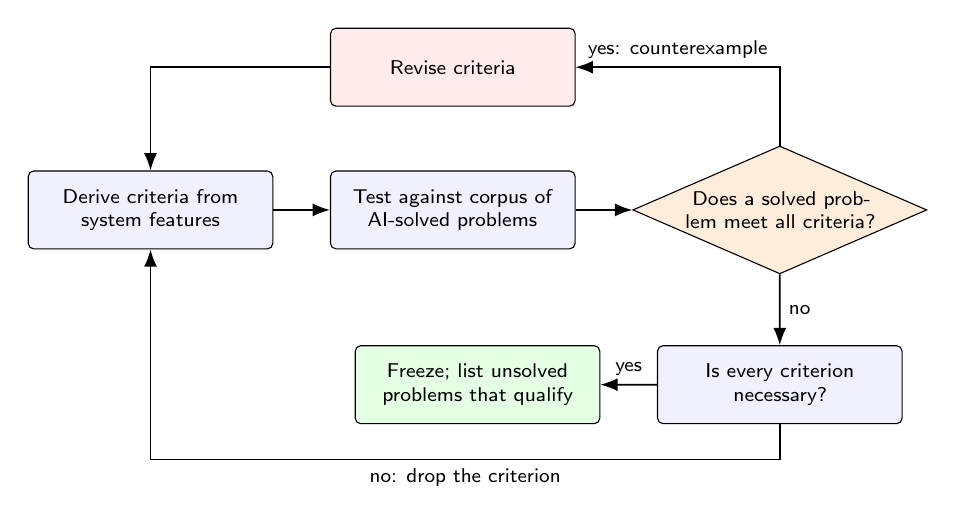
\begin{tikzpicture}[node distance=6mm and 8mm, font=\footnotesize\sffamily, scale=0.9, transform shape,
 box/.style={draw, rounded corners=2pt, align=center, inner sep=5pt, fill=blue!6, text width=31mm, minimum height=11mm},
 dec/.style={draw, diamond, aspect=2.3, align=center, inner sep=1pt, fill=orange!14, text width=27mm},
 arr/.style={-{Latex[length=2.2mm]}, semithick}]
\node[box] (a) {Derive criteria from\\ system features};
\node[box, right=of a] (b) {Test against corpus of\\ AI-solved problems};
\node[dec, right=of b] (c) {Does a solved problem meet all criteria?};
\node[box, below=10mm of c] (d) {Is every criterion\\ necessary?};
\node[box, left=of d, fill=green!10] (e) {Freeze; list unsolved\\ problems that qualify};
\node[box, above=9mm of b, fill=red!8] (f) {Revise criteria};
\draw[arr] (a) -- (b);
\draw[arr] (b) -- (c);
\draw[arr] (c) -- node[right, font=\footnotesize\sffamily]{no} (d);
\draw[arr] (d) -- node[above, font=\footnotesize\sffamily]{yes} (e);
\draw[arr] (c.north) |- node[pos=0.75, above, font=\footnotesize\sffamily]{yes: counterexample} (f.east);
\draw[arr] (f.west) -| (a.north);
\draw[arr] (d.south) -- ++(0,-5mm) -| node[pos=0.25, below, font=\footnotesize\sffamily]{no: drop the criterion} (a.south);
\end{tikzpicture}
\caption{The falsification loop. A version of the criteria survives only if no reported AI solution meets all of its criteria.}\label{fig:loop}
\end{figure}

\subsection{Test corpus}

Table~\ref{tab:corpus} lists the reported AI solutions used as the test set. ``Solved'' includes claims that are not yet verified, and solutions obtained by humans working with AI. This is deliberate: counting claims makes the test stricter for the criteria.

\begin{table}[!htb]
\centering\footnotesize
\begin{tabularx}{\textwidth}{L{4.6cm} L{2.5cm} Y}
\toprule
Source & Items & Status and handling\\
\midrule
OpenAI mathematics release, 6~Oct 2026; catalogue as of 21~Nov 2026 \cite{openairelease,openairepo} & 373 result families, 721 manuscripts & Company preprints. 245 families (66\%) carry a Lean formalisation tag in the catalogue; three manuscripts were withdrawn after an error \cite{kingy}. Each family assessed from its catalogue summary.\\
Riemann Hypothesis and GRH, L.~Alp\"oge with Claude, 20~Nov 2026 \cite{rhscience,rhdev} & 1 & Released as 17.4 million lines of Lean; compiled independently; the argument has not been digested by mathematicians. Assessed individually.\\
Navier--Stokes blow-up with forcing, OpenAI, 8~Sep 2026 \cite{nsopenai,nsnature} & 1 & Lean formalisation published; acceptance by the community is pending. Assessed individually.\\
Unit distance conjecture, OpenAI, 20~May 2026 \cite{udopenai,udremarks} & 1 & Disproof; human-verified digest available. Assessed individually.\\
Formal proof search on Erd\H{o}s problems \cite{nexus} & 9 problems & Lean proofs. Assessed as a group, using the database curator's characterisation \cite{fme}.\\
Added during write-up: Jacobian conjecture counterexample (Jul 2026) \cite{fme}, irrationality of $\zeta(5)$ (human + AI) \cite{fmapery}, five resolutions in FrontierMath Erd\H{o}s \cite{fme} & 7 & Mixed status. Assessed individually after the criteria were frozen; none changed the result.\\
qtBench proposals by internal OpenAI models \cite{combi}; added on 22~Nov 2026 & 21 proposals & The benchmark authors consider 10 genuine and found that at least 4 rely on gaming the checker; the rest is under assessment. Assessed as a group from the paper's description.\\
\bottomrule
\end{tabularx}
\caption{Test corpus of reported AI solutions.}\label{tab:corpus}
\end{table}

\subsection{Checking procedure}

All checks were made by the AI model within one working session. For each item it compared the problem with the criteria, using the catalogue summary of the result and its own knowledge of the earlier literature. For the cases that came closest to meeting the criteria it ran web searches on the history of the problem and on the verification status of the claim. Each of the 373 families was also classified by result type (general proof, quantitative or algorithmic result, construction or counterexample); the classification is given in Appendix~\ref{app:ids}.

Three things were \emph{not} done. The 721 manuscripts were not read. The prior partial result identified for each family was not recorded family by family. No second rater repeated the assessment. Section~\ref{sec:limits} returns to these points.

The reference list was checked against publisher, arXiv or archive records on 22~November 2026. One entry whose author could not be confirmed was replaced, and one byline that could not be confirmed was removed. The classical results that Tables~\ref{tab:hard} and~\ref{tab:screen} cite by author and year were checked only in part.

\section{The six versions of the criteria}\label{sec:versions}

Figure~\ref{fig:versions} and Table~\ref{tab:versions} summarise the path from eight criteria to two.

\begin{figure}[!htb]
\centering
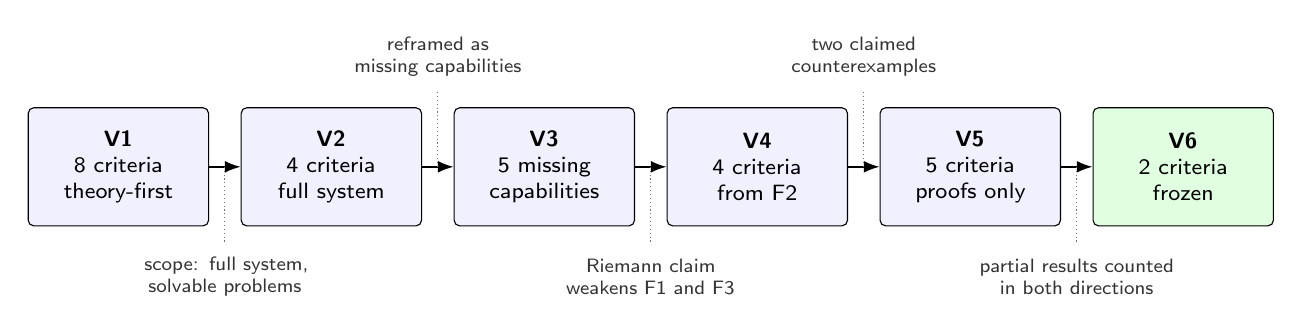
\begin{tikzpicture}[font=\footnotesize\sffamily, node distance=4mm,
 v/.style={draw, rounded corners=2pt, align=center, minimum height=15mm, text width=21.5mm, inner sep=2pt, fill=blue!6},
 ev/.style={align=center, text width=34mm, font=\scriptsize\sffamily, text=black!80},
 arr/.style={-{Latex[length=2mm]}, semithick}]
\node[v] (v1) {\textbf{V1}\\ 8 criteria\\ theory-first};
\node[v, right=of v1] (v2) {\textbf{V2}\\ 4 criteria\\ full system};
\node[v, right=of v2] (v3) {\textbf{V3}\\ 5 missing\\ capabilities};
\node[v, right=of v3] (v4) {\textbf{V4}\\ 4 criteria\\ from F2};
\node[v, right=of v4] (v5) {\textbf{V5}\\ 5 criteria\\ proofs only};
\node[v, right=of v5, fill=green!12] (v6) {\textbf{V6}\\ 2 criteria\\ frozen};
\foreach \a/\b in {v1/v2,v2/v3,v3/v4,v4/v5,v5/v6} \draw[arr] (\a) -- (\b);
\node[ev] at ($(v1)!0.5!(v2)+(0,-14mm)$) {scope: full system,\\ solvable problems};
\node[ev] at ($(v2)!0.5!(v3)+(0,14mm)$) {reframed as\\ missing capabilities};
\node[ev] at ($(v3)!0.5!(v4)+(0,-14mm)$) {Riemann claim\\ weakens F1 and F3};
\node[ev] at ($(v4)!0.5!(v5)+(0,14mm)$) {two claimed\\ counterexamples};
\node[ev] at ($(v5)!0.5!(v6)+(0,-14mm)$) {partial results counted\\ in both directions};
\foreach \a/\b/\s in {v1/v2/-1,v2/v3/1,v3/v4/-1,v4/v5/1,v5/v6/-1} \draw[densely dotted, black!55] ($(\a)!0.5!(\b)$) -- ($(\a)!0.5!(\b)+(0,\s*9.5mm)$);
\end{tikzpicture}
\caption{Versions of the criteria and the event that triggered each revision.}\label{fig:versions}
\end{figure}

\begin{table}[!htb]
\centering\footnotesize
\begin{tabularx}{\textwidth}{L{0.7cm} L{5.3cm} L{3.3cm} Y}
\toprule
 & Criteria & Tested against & Outcome\\
\midrule
V1 & (1) no general method can exist; (2) independent of the axioms; (3) only exhaustive search known; (4) many dependent steps; (5) too much to hold at once; (6) no cheap check; (7) far from existing mathematics; (8) self-reference & Theory and three early results \cite{udopenai,nexus,nsopenai} & 1--3 also stop humans; 4--6 bind only a bare model; 7 unproven and already under pressure; 8 artificial.\\
V2 & Infeasible exact computation; self-reference; known methods provably fail; no measurable partial progress & None (scope revision) & No criterion was at once proven, specific to LLMs and mathematically interesting.\\
V3 & Capabilities F1--F5 of Section~\ref{sec:background} & Riemann Hypothesis claim & F1 and F3 weakened; F4 supplied by the proof checker; F5 artificial; F2 retained.\\
V4 & Precise and not known undecidable; seriously attempted; no stepping stone toward the solution; no score & Four results, then all 373 families & No counterexample among general proofs; two claimed counterexamples among constructions.\\
V5 & V4 plus ``a general proof is required'' & 373 families & No counterexample, but no prediction for problems settled by an example.\\
V6 & Scope condition; \Cone{} prominent; \Ctwo{} no partial result in either direction & 373 families and 10 further results & No counterexample; both criteria necessary. Frozen.\\
\bottomrule
\end{tabularx}
\caption{The six versions. ``Stepping stone'' in V4 meant a proven non-trivial weaker statement that would follow from the solution; ``score'' meant a number that measures how close an attempt is.}\label{tab:versions}
\end{table}

\paragraph{V1 to V2.} The first list mixed three kinds of limits. Limits of all computation (undecidability, independence, infeasible search) hold for every solver and therefore say nothing specific about LLMs. Limits of the bare transformer (depth, context, error accumulation) are real \cite{ms24,cpw}, but code execution, external memory and a proof checker remove them. The remaining criterion, distance from existing mathematics, could not be tested before a problem is solved.

\paragraph{V2 to V3.} The author restated the aim: the criteria should name capabilities that a problem requires and that LLMs lack. This produced F1--F5.

\paragraph{V3 to V4.} On 20~November a proof of the Riemann Hypothesis, found with an LLM and released as formal code, was announced \cite{rhscience}. The Riemann Hypothesis was a standard example of a problem expected to need new ideas, so the claim counts against F1 and F3 as criteria: whatever the system lacks in these two respects did not put the problem out of reach. What was released is 17.4 million lines of formal code \cite{rhdev}, not a readable theory. F2 was not contradicted, because the problem had a long record of partial results, the latest being a zero-free half-plane $\Re s>7/8$ claimed one month earlier \cite{openairepo}. The author then imposed the falsification condition, and V4 was built on F2 alone.

\paragraph{V4 to V5.} A spot check of four results found no counterexample, since each had a stepping stone or a score. The full pass over the October release then found two claimed disproofs that appeared to meet all four criteria: the Lipman--Zariski conjecture (open since 1965) and Zariski's multiplicity conjecture (1971). In both cases every earlier partial result that the model knew of \emph{supported} the conjecture, so there was no stepping stone toward the counterexample. Neither claim is verified \cite{nakai,sampaio}. V5 removed them by restricting the claim to general proofs.

\paragraph{V5 to V6.} The author asked for the minimum set. Counting partial results in \emph{either} direction makes the fifth criterion unnecessary: both conjectures had been proven in infinite families of cases \cite{graf,hochster,greuel}, and such results narrow where a counterexample can lie. A proven bound is itself a weaker statement, so ``no score'' merges with ``no partial result''. ``Seriously attempted'' was restated as ``prominent'', which can be checked from surveys and problem lists.

\FloatBarrier
\section{Results}\label{sec:results}

Table~\ref{tab:metrics} collects the main numbers. The subsections explain them.

\begin{table}[!htb]
\centering\footnotesize
\begin{tabular}{L{8.6cm} r}
\toprule
Metric & Value\\
\midrule
Versions of the criteria; number of criteria in the first and last version & 6; 8 and 2\\
Result families in the main corpus (manuscripts) & 373 (721)\\
\quad of which general proofs / quantitative / constructions & 232 / 64 / 77\\
\quad of which with a Lean tag in the catalogue & 245 (66\%)\\
Further reported results assessed individually & 10\\
Reported solutions assessed as groups (Erd\H{o}s problems; qtBench) & 9; 10\\
Claimed counterexamples to V4, V5, V6 & 2, 0, 0\\
FrontierMath Erd\H{o}s conjectures reported resolved within three months & 16 of 68 (24\%)\\
Open problems screened against the frozen criteria; qualifying & 26; 5\\
Qualifying problems with a Lean statement in Formal Conjectures & 4 of 5\\
\bottomrule
\end{tabular}
\caption{Summary of metrics.}\label{tab:metrics}
\end{table}

\subsection{Composition of the main corpus}

Figure~\ref{fig:area} shows the 373 result families by area and result type. By our classification, 232 families (62\%) are general proofs of qualitative statements, 64 (17\%) are quantitative or algorithmic results, and 77 (21\%) are constructions, counterexamples or independence results. A Lean tag is present for 58\% of the general proofs, 83\% of the quantitative results and 74\% of the constructions. During the session a keyword count had estimated the share of constructions at 23\%; the manual classification replaces that figure.

\begin{figure}[!htb]
\centering
% --- chart data (generated from the classification in Appendix A) ---
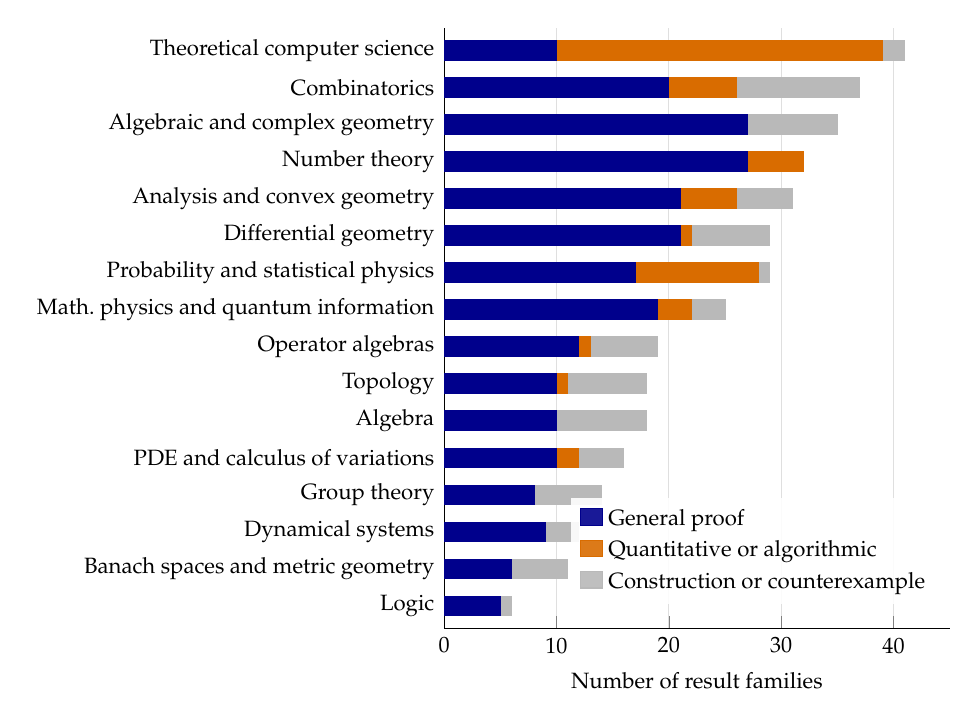
\begin{tikzpicture}
\begin{axis}[xbar stacked, width=0.66\textwidth, height=9.2cm, bar width=7pt,
ytick={0,1,2,3,4,5,6,7,8,9,10,11,12,13,14,15}, yticklabels={{Logic},{Banach spaces and metric geometry},{Dynamical systems},{Group theory},{PDE and calculus of variations},{Algebra},{Topology},{Operator algebras},{Math.\ physics and quantum information},{Probability and statistical physics},{Differential geometry},{Analysis and convex geometry},{Number theory},{Algebraic and complex geometry},{Combinatorics},{Theoretical computer science}}, yticklabel style={font=\footnotesize}, xticklabel style={font=\footnotesize},
xmin=0, xmax=45, xlabel={\footnotesize Number of result families}, enlarge y limits=0.04, axis lines*=left, xmajorgrids, grid style={gray!25},
legend style={at={(0.98,0.04)},anchor=south east,font=\footnotesize,draw=none,fill=white,fill opacity=0.9,text opacity=1}, legend cell align=left, reverse legend=false]
\addplot+[fill=blue!55!black,draw=blue!55!black] coordinates {(5,0) (6,1) (9,2) (8,3) (10,4) (10,5) (10,6) (12,7) (19,8) (17,9) (21,10) (21,11) (27,12) (27,13) (20,14) (10,15)};
\addlegendentry{General proof}
\addplot+[fill=orange!85!black,draw=orange!85!black] coordinates {(0,0) (0,1) (0,2) (0,3) (2,4) (0,5) (1,6) (1,7) (3,8) (11,9) (1,10) (5,11) (5,12) (0,13) (6,14) (29,15)};
\addlegendentry{Quantitative or algorithmic}
\addplot+[fill=gray!55,draw=gray!55] coordinates {(1,0) (5,1) (3,2) (6,3) (4,4) (8,5) (7,6) (6,7) (3,8) (1,9) (7,10) (5,11) (0,12) (8,13) (11,14) (2,15)};
\addlegendentry{Construction or counterexample}
\end{axis}
\end{tikzpicture}

\caption{The 373 result families of the October release by area and result type. Areas follow the order of the catalogue \cite{openairepo}; the grouping and the type classification are ours (Appendix~\ref{app:ids}).}\label{fig:area}
\end{figure}

\subsection{Matching results by version}

\begin{table}[!htb]
\centering\footnotesize
\begin{tabularx}{\textwidth}{l L{4.3cm} r r Y}
\toprule
Version & Test set & Items & Counterexamples & Remark\\
\midrule
V3 & Riemann Hypothesis claim & 1 & -- & contradicts 2 of 5 capabilities\\
V4 & spot check & 4 & 0 & each result had a stepping stone or a score\\
V4 & October release & 373 & 2 & 0.5\% of families; 2.6\% of the 77 constructions\\
V5 & October release & 373 & 0 & constructions out of scope\\
V6 & release and 3 individual results & 376 & 0 & closest call: Gaussian moat conjecture\\
V6 & additions during write-up & 7 & 0 & Jacobian, $\zeta(5)$, five FrontierMath Erd\H{o}s resolutions\\
V6 & qtBench solutions judged genuine & 10 & 0 & assessed as a group; recent, specialised problems\\
\bottomrule
\end{tabularx}
\caption{Counterexamples found per version. The nine Erd\H{o}s problems of \cite{nexus} were assessed as a group and are not listed. The qtBench solutions \cite{combi} were also assessed as a group and were added after the freeze.}\label{tab:matching}
\end{table}

Table~\ref{tab:matching} gives the counts. Under V6, the 64 quantitative families fail \Ctwo{} almost by definition: they improve or settle a bound, a rate or a running time for which earlier results existed. For the general proofs and the constructions, the model went through the families one by one and in each case either recalled a proven special case, a weaker form or a bound that predated the AI result, or inferred one from the catalogue description. These recollections were not recorded (Section~\ref{sec:limits}). Table~\ref{tab:hard} lists the cases where the verdict was least obvious.

\begin{table}[!htb]
\centering\footnotesize
\begin{tabularx}{\textwidth}{L{3.9cm} Y L{2.5cm}}
\toprule
Reported result & Partial results that existed before & Verdict under V6\\
\midrule
Riemann Hypothesis \cite{rhscience} & Zero-free regions (de la Vall\'ee Poussin 1899; Vinogradov and Korobov 1958); a positive proportion of zeros on the critical line (Selberg 1942; Levinson 1974; Conrey 1989); zero-free half-plane claimed in Oct 2026 & fails \Ctwo\\
Irrationality of Catalan's constant \cite{openairepo} & At least one of seven related constants is irrational (Rivoal and Zudilin 2003) & fails \Ctwo\\
Irrationality exponent of $\pi$ equals 2 \cite{openairepo} & Upper bounds 42 (Mahler 1953), 7.61 (Salikhov 2008), 7.10 (Zeilberger and Zudilin 2020) & fails \Ctwo\\
Irrationality of $\zeta(5)$ \cite{fmapery} & One of $\zeta(5),\zeta(7),\zeta(9),\zeta(11)$ is irrational (Zudilin 2001) & fails \Ctwo\\
Unit distance conjecture \cite{udopenai} & Lower bound of Erd\H{o}s (1946); upper bound $O(n^{4/3})$ (Spencer, Szemer\'edi and Trotter 1984) & fails \Ctwo\\
Thompson's group $F$ is non-amenable \cite{openairepo,kimlodha} & No free subgroups (Brin and Squier 1985); fast growth of the F\o lner function (Moore 2013); non-amenability of a finitely presented group containing $F$ (Lodha and Moore 2016) & fails \Ctwo\\
Positive entropy of the standard map \cite{openairepo} & Hyperbolic sets of Hausdorff dimension close to 2 for large parameters (Duarte 1994; Gorodetski 2012) & fails \Ctwo\\
Navier--Stokes blow-up with forcing \cite{nsopenai} & Global regularity for small data (Fujita and Kato 1964); partial regularity (Caffarelli, Kohn and Nirenberg 1982) & fails \Ctwo\\
Jacobian conjecture, counterexample \cite{fme} & Degree 2 (Wang 1980); reduction to degree 3 (Bass, Connell and Wright 1982) & fails \Ctwo\\
Lipman--Zariski, counterexample \cite{openairepo} & True for hypersurfaces, complete intersections, graded rings and log canonical singularities \cite{graf,hochster} & met V4; fails \Ctwo\\
Zariski multiplicity, counterexample \cite{openairepo} & True for curves and weighted homogeneous singularities \cite{greuel} & met V4; fails \Ctwo\\
Gaussian moat conjecture \cite{openairepo} & Computed moats up to width 6 \cite{tsuchimura}; the conjecture for step sizes $\sqrt2$ and $2$ \cite{gethnerstark}; prime-free neighbourhoods of arbitrary radius around a Gaussian prime & fails \Ctwo{} (closest call)\\
\bottomrule
\end{tabularx}
\caption{The reported results that came closest to meeting the criteria. Classical results are cited by author and year only.}\label{tab:hard}
\end{table}

The Gaussian moat conjecture, posed in 1962, is the closest call. Its record was almost entirely computational, and finite computations do not count under \Ctwo. Two theoretical results existed. For every radius there is a Gaussian prime with no other Gaussian prime within that radius. Gethner and Stark also proved, with a device that they called periodic moats, that no walk to infinity exists from any starting point for the step sizes $\sqrt2$ and $2$ \cite{gethnerstark}. Both are weaker forms of the conjecture, and the reported proof builds a periodic sieve obstruction \cite{openairepo}, which is in the spirit of the second. We counted them as partial results. A reader who regards them as too slight would count the moat conjecture as a counterexample to V6.

\subsection{Why two criteria, and why both}

\paragraph{\Ctwo{} is necessary.} Without it, any prominent problem qualifies, and the Riemann Hypothesis is then a counterexample.

\paragraph{\Cone{} is necessary.} Without it, a problem qualifies whenever nothing has been proven about it, and that is also true of problems nobody has worked on. The curator of the Erd\H{o}s problems database reports that many AI-solved Erd\H{o}s problems were obscure and yielded to straightforward modifications of known techniques, while the famous ones that fell had been the subject of numerous papers and partial results \cite{fme}.

\paragraph{Nothing else is needed.} The other criteria of V4 and V5 either merge into \Ctwo{} (a bound is a partial result; a special case in the opposite direction is a hint for a construction) or were contradicted by the evidence (F1, F3). No counterexample to the pair was found, so no further criterion is required by the falsification condition.

\paragraph{Why the pair is plausible.} Both training and proof search depend on intermediate signals: a statement that can be proven on the way, a quantity that can be improved, a restricted case that can be checked. In our assessment, every prominent problem in the corpus that was reported solved had such signals available in the literature. The pair \Cone{}, \Ctwo{} describes problems where the literature offers none, although specialists have looked. This is capability F2 of Section~\ref{sec:background}, stated as a property of the problem.

\paragraph{A property outside the pair.} The qtBench results (Section~\ref{sec:crosschecks}) add a lesson that the pair does not capture. The problems of that benchmark were chosen so that no incremental contribution exists: a proposed rule either reproduces the data exactly or it does not \cite{combi}. About a third of them were nevertheless solved once a system could generate candidate rules and test each one by computation. The absence of partial progress is therefore not sufficient when candidates can be tested mechanically. The five problems of Section~\ref{sec:final} do not allow such tests: a solution is a general proof, and a computation can confirm only finitely many cases. This is the ``no score'' criterion of V4 in a sharper form. Under the freeze rule we do not add it as a third criterion. We record it as a property that the five problems share and that a future revision of the criteria should test.

\subsection{External cross-checks}\label{sec:crosschecks}

\paragraph{FrontierMath Erd\H{o}s.} This benchmark consists of 68 conjectures selected in August 2026 by the database curator as the most difficult and interesting open Erd\H{o}s problems \cite{fme}. The benchmark's own runs resolved 5 of them, 2 within the controlled budget. By our matching of descriptions (Appendix~\ref{app:fme}), 11 more are covered by claims in the October release. If the claims hold, 16 of 68 (24\%) fell within about three months of the selection. Expert judgement of difficulty was therefore a weak predictor. None of the five problems of Section~\ref{sec:final} is among the 68.



\paragraph{Benchmarks of checkable objects.} FrontierMath: Open Problems lists 49 problems, of which 5 are marked solved by AI, 5 by humans with AI, and 39 unsolved \cite{fmop}. It and HorizonMath \cite{horizon} admit only problems whose solution is a concrete object that a program can verify, so the five problems of Section~\ref{sec:final}, which need general proofs, cannot appear in them. One entry is close: a problem on Ap\'ery-style irrationality proofs with targets $\zeta(5)$, $\zeta(7)$, Catalan's constant, the Calegari--Dimitrov--Tang constant and Euler's constant \cite{fmapery}. Two targets have fallen, both with earlier partial results; $\pi+e$ is not a target.

\paragraph{qtBench.} This benchmark contains 29 open problems in algebraic combinatorics that ask for a simple rule, a statistic or a bijection, which explains given polynomial data \cite{combi}. Its authors expected public models to solve none of them, and in their baseline runs of two hours per problem no proposal of a public model passed their checks. Internal OpenAI models then returned proposals for 21 problems. The authors consider 10 of them genuine solutions, among them three counterexamples to positivity conjectures, and they found that at least 4 rely on gaming the checker. We added the 10 solutions to the test corpus on 22~November, after the freeze. In our assessment none of them meets the pair. By the benchmark's own description these are recent questions from a specialised literature, some of them posed only informally, so they fail \Cone. The one decades-old problem in the benchmark, a bijection that exchanges area and bounce on Dyck paths, has documented partial results and therefore fails \Ctwo; the proposal for it had not been assessed when the paper appeared.

\paragraph{Formal Conjectures.} This repository of Lean statements \cite{fc} contains four of our five problems as open statements, and three of them belong to its fixed 100-problem evaluation sets (Table~\ref{tab:final}). The repository also classifies the fact that $\pi+e$ or $\pi e$ is transcendental as textbook level, and the corresponding fact for Euler's constant and Gompertz's constant as a research result. This agrees with our line between trivial and non-trivial partial results.

\FloatBarrier
\section{The frozen criteria and the problems that meet them}\label{sec:final}

The criteria were frozen on 21~November 2026 in the following wording.

\begin{center}
\fbox{\begin{minipage}{0.93\textwidth}\vspace{2pt}
\textbf{Scope.} The problem is a precise statement that is not known to be undecidable.\\[3pt]
\Cone{} \textbf{Prominent.} Specialists have known the problem for decades, so missing progress is not due to neglect.\\[3pt]
\Ctwo{} \textbf{No partial result.} Nobody has proven a non-trivial weaker form of the statement or of its opposite: no infinite family of cases, no weaker conclusion and no bound. Checking finitely many cases by computer does not count.\\[3pt]
\textbf{Rule.} A solution of any qualifying problem by an AI system refutes the pair. The pair is not adjusted afterwards.\vspace{2pt}
\end{minipage}}
\end{center}

Two operational notes were applied but are not part of the frozen text: a conditional implication (the statement follows from another open conjecture) is not a partial result, and neither is a theorem about a different object. The five problems below are the outcome of one screening pass. The list is not claimed to be complete, and to our knowledge all five were open on the date of the freeze.

\begin{problem}[Sum and product of $\pi$ and $e$]
Is $\pi+e$ irrational? Is $\pi e$ irrational?
\end{problem}
\noindent Both numbers are individually transcendental (Hermite 1873; Lindemann 1882). Since $\pi$ and $e$ are the roots of $x^2-(\pi+e)x+\pi e$, at least one of $\pi+e$ and $\pi e$ is transcendental; this two-line argument is all that is known. Related numbers are understood, for example $e^{\pi}$ (Gelfond 1934) and the pair $\pi$, $e^{\pi}$ \cite{nesterenko}, but no method produces rational approximations to $\pi+e$ of the quality an irrationality proof needs \cite{dkz}.

\begin{problem}[Non-Wieferich primes]
Are there infinitely many primes $p$ with $2^{\,p-1}\not\equiv 1 \pmod{p^2}$?
\end{problem}
\noindent Only two primes with $2^{\,p-1}\equiv 1 \pmod{p^2}$ are known, 1093 and 3511, and searches beyond $6\times10^{15}$ have found no other. Yet it is not known that infinitely many primes fail the congruence, and all non-computational results are conditional \cite{gm}: the statement follows from the $abc$ conjecture \cite{silverman} and from a strong form of Erd\H{o}s problem~11 \cite{gs}. The second implication is a route by which the problem could fall as a by-product.

\begin{problem}[Mersenne primes]
Are there infinitely many primes $p$ such that $2^p-1$ is prime?
\end{problem}
\noindent Fifty-two such primes are known. It is equally unknown whether $2^p-1$ is composite for infinitely many primes $p$ \cite{mersennewiki}. A conditional theorem shows that $a^p-b$ is composite for almost all primes $p$, and the pair $(a,b)=(2,1)$ is exactly the case that it excludes \cite{jt}. Lower bounds for the largest prime factor of $2^n-1$ exist, but they are not weaker forms of either statement.

\begin{problem}[Fermat primes]
Is $F_n=2^{2^n}+1$ composite for every $n\ge 5$?
\end{problem}
\noindent $F_0,\dots,F_4$ are prime and $F_5,\dots,F_{32}$ are composite. It is unknown whether infinitely many $F_n$ are prime, and unknown whether infinitely many are composite.

\begin{problem}[Gilbreath's conjecture]
Let $d_0(n)=p_n$ be the $n$-th prime and $d_k(n)=\lvert d_{k-1}(n+1)-d_{k-1}(n)\rvert$ for $k\ge1$. Is $d_k(1)=1$ for every $k\ge 1$?
\end{problem}
\noindent The conjecture has been verified by computer far beyond the range of Odlyzko's 1993 computation \cite{odlyzko}, but nothing has been proven about it for the primes. The existing theorems concern random analogues \cite{chase,cht}. The second of these papers, from July 2026, also gives a deterministic analysis that isolates the possible obstructions under an unproven bound on prime gaps. Under our operational notes neither is a partial result, because one concerns a different object and the other is conditional. A specialist could judge this differently, which makes Problem~5 the entry most open to dispute.

\begin{table}[!htb]
\centering\footnotesize
\begin{tabularx}{\textwidth}{L{2.6cm} L{6.6cm} Y}
\toprule
Problem & Lean statement in Formal Conjectures \cite{fc} & Evaluation set\\
\midrule
1. $\pi+e$, $\pi e$ & \texttt{irrational\_e\_plus\_pi}, \texttt{irrational\_e\_times\_pi} & --\\
2. Non-Wieferich & only as conclusion of a conditional theorem under Erd\H{o}s problem 11 & --\\
3. Mersenne & \texttt{infinitely\_many\_mersenne\_primes} & FC100OpenSet2\\
4. Fermat & \texttt{fermat\_number\_are\_composite}, \texttt{infinite\_fermat\_primes}, \texttt{infinite\_fermat\_composite} & FC100OpenSet2 (second statement)\\
5. Gilbreath & \texttt{gilbreath\_conjecture} & FC100OpenSet1\\
\bottomrule
\end{tabularx}
\caption{Formal statements of the five problems, as found in the repository on 21~November 2026.}\label{tab:final}
\end{table}

\subsection{Open problems that do not qualify}

Table~\ref{tab:screen} lists well-known open problems that we screened and rejected, with the partial result that excludes them. The table shows how selective \Ctwo{} is: most famous problems have a rich record of partial results, and the criteria make no prediction about them.

{\footnotesize
\begin{longtable}{L{4.2cm} L{11.0cm}}
\toprule
Open problem & Partial result that excludes it under \Ctwo\\
\midrule
\endfirsthead
\toprule
Open problem (continued) & Partial result that excludes it under \Ctwo\\
\midrule
\endhead
\midrule
\multicolumn{2}{r}{\emph{continued on the next page}}\\
\endfoot
\bottomrule
\addlinespace[6pt]
\caption{Screened open problems that fail \Ctwo. Classical results are cited by author and year only.}\label{tab:screen}
\endlastfoot
P versus NP & Lower bounds for restricted circuit classes (Razborov 1985; H\aa stad 1986)\\
Collatz conjecture & Almost all orbits attain almost bounded values (Tao 2022)\\
Twin prime conjecture & Infinitely many prime gaps of at most 246 (Zhang 2014; Maynard 2015; Polymath 2014)\\
Goldbach conjecture & Every large even number is a prime plus a product of at most two primes (Chen 1973)\\
Odd perfect numbers & None below $10^{1500}$ (Ochem and Rao 2012)\\
Primes of the form $n^2+1$ & $n^2+1$ has at most two prime factors infinitely often (Iwaniec 1978)\\
Irrationality of Euler's constant $\gamma$ & $\gamma$ or Gompertz's constant is irrational (Aptekarev 2009), indeed transcendental (Rivoal 2012)\\
Irrationality of $e^{e}$ & $e^{e}$ or $e^{e^2}$ is transcendental \cite{brownawell}\\
Algebraic independence of $e$ and $\pi$ & They are independent or $e^{\pi^2}$ is transcendental \cite{brownawell}\\
Irrationality of $\zeta(7)$ & One of $\zeta(5),\dots,\zeta(11)$ is irrational (Zudilin 2001)\\
Linear independence of zeta zeros & The zeros contain no infinite arithmetic progression (Putnam 1954)\\
Infinitely many regular primes & Infinitely many irregular primes (Jensen 1915), a weaker form of the opposite\\
Brocard's problem $n!+1=m^2$ & Solved when $m$ is restricted to certain recurrence sequences \cite{bravo}\\
Erd\H{o}s--Straus conjecture & Holds for almost all $n$ (Vaughan 1970)\\
$abc$ conjecture & Exponential bounds (Stewart and Yu 2001)\\
Schanuel's conjecture & Lindemann--Weierstrass theorem; Baker's theorem\\
Hodge conjecture & Lefschetz theorem on $(1,1)$ classes\\
Birch and Swinnerton-Dyer conjecture & Analytic rank at most one (Gross and Zagier 1986; Kolyvagin 1990)\\
Navier--Stokes regularity without forcing & Partial regularity (Caffarelli, Kohn and Nirenberg 1982)\\
Yang--Mills mass gap & Lattice theory at strong coupling (Osterwalder and Seiler 1978)\\
Normality of $\pi$ & Borderline: nothing is known about digit frequencies, but bounds on the irrationality exponent limit runs of a single digit. Not listed.\\
\end{longtable}}

\FloatBarrier
\section{Related work}

Three kinds of work are close to ours. Benchmarks of unsolved problems select by expert judgement and by verifiability \cite{fmop,horizon,fme,fc}. One benchmark in algebraic combinatorics, qtBench, was built on a hypothesised weakness of LLMs, a tendency toward what its authors call ``low-entropy'' thinking \cite{combi}. The hypothesis resembles our capability F3 and met the same fate: internal OpenAI models produced what the authors consider genuine solutions to 10 of its 29 open problems (Section~\ref{sec:crosschecks}). An earlier study of bijection discovery with an evolutionary LLM system had not solved the open problem it targeted \cite{brown}. Finally, mathematicians have described the reporting bias of the field: successes are announced and failures are not, so success rates are unknown \cite{taoicm,fme}. We found no work that derives criteria from system features, tests them by falsification and freezes a list of predicted survivors.

\section{Limitations}\label{sec:limits}

\begin{itemize}
\item \textbf{Single AI rater.} All judgements were made by one AI model from catalogue summaries and from its own knowledge of the literature, which is uneven across fields. A specialist could overturn individual judgements, in particular what counts as a non-trivial partial result.
\item \textbf{Undocumented per-family evidence.} The partial result behind each of the 373 verdicts was not recorded, except for the cases in Table~\ref{tab:hard}. An audit would have to repeat the pass.
\item \textbf{Unverified claims.} By the company's count of 7~October, 300 of 719 released results had a Lean formalisation \cite{kingy}; the catalogue tag used in Table~\ref{tab:corpus} is per family and may cover only part of a family. Several headline claims are disputed or not yet accepted. In the one batch of AI proposals that specialists have assessed in detail, 10 of 21 were judged genuine and at least 4 relied on gaming the checker \cite{combi}. Counting claims as solutions is conservative for the criteria but makes the corpus noisy.
\item \textbf{Successes only.} The problems that AI systems attempted and failed are not published \cite{taoicm}. The criteria could be tested against successes, not against failures. One exception is documented: OpenAI reports that it set its system on the open Millennium Prize problems in September 2026, and it announced a solution only for Navier--Stokes \cite{nsopenai}.
\item \textbf{Incomplete corpus.} The corpus is not a complete list of reported AI solutions. For example, a reported result on complex structures on the six-dimensional sphere \cite{sixsphere} was found only during the reference check and was not assessed in detail; that problem has known partial results, so it would fail \Ctwo.
\item \textbf{Narrowness and base rates.} \Ctwo{} is strict. Few problems meet it, so the absence of counterexamples carries limited weight: problems without any partial result are rare among solved problems of any origin.
\item \textbf{Hard for everyone.} The five problems are also out of reach for human mathematicians. The criteria do not separate machines from humans; they describe problems where no solver has a foothold.
\item \textbf{Risk of fitting.} The criteria were revised after seeing the data. The freeze and the refutation rule are the safeguard: from 21~November 2026 the list is a prediction.
\end{itemize}

\FloatBarrier
\section{Conclusion}

Starting from eight criteria, the falsification loop removed everything that was an architectural limit of the bare model, everything that concerned novelty, and everything that distinguished proofs from constructions. What remained is one property, stated twice: the literature offers no foothold (\Ctwo), and this is not for lack of trying (\Cone). Among 373 result families and the further reported results of Table~\ref{tab:corpus} we found no AI solution of a problem with that property, and we found five unsolved problems that have it. The claim is modest and testable: if an AI system proves, for example, that $\pi+e$ is irrational or that infinitely many primes are not Wieferich primes, the criteria are refuted.

\section*{AI disclosure}

This paper was produced in a working session between the author and Claude, an AI model developed by Anthropic. The author conceived the question, set the scope decisions and the falsification rule, and directed the iterations. The AI model carried out the web searches, the corpus checks, the classification of the 373 result families and the screening of open problems, and it drafted the text, the tables and the figures. Its judgements have not been verified independently (Section~\ref{sec:limits}). Two results in the test corpus, the Riemann Hypothesis claim and the Jacobian counterexample, were reported by an Anthropic researcher working with Claude models; they were assessed from public reports only.

\begingroup
\small
\begin{thebibliography}{99}\setlength{\itemsep}{1pt}
\bibitem{udopenai} OpenAI. An OpenAI model has disproved a central conjecture in discrete geometry. 20 May 2026. \url{https://openai.com/index/model-disproves-discrete-geometry-conjecture/}
\bibitem{udremarks} N.~Alon, T.~F.~Bloom, W.~T.~Gowers, D.~Litt, W.~Sawin, A.~Shankar, J.~Tsimerman, V.~Wang, M.~M.~Wood. Remarks on the disproof of the unit distance conjecture. arXiv:2605.20695, 2026.
\bibitem{nexus} G.~Tsoukalas, A.~Kovsharov, S.~Shirobokov, et al. Advancing mathematics research with AI-driven formal proof search. arXiv:2605.22763; \emph{Science}, 2026, doi:10.1126/science.aej2213.
\bibitem{nsopenai} OpenAI. On the Navier--Stokes Millennium Prize Problem. 8 September 2026. \url{https://openai.com/index/navier-stokes-solution/}
\bibitem{nsnature} OpenAI claims huge maths breakthrough on a famed `Millennium Problem'. \emph{Nature} (news), 8 September 2026. \url{https://www.nature.com/articles/d41586-026-02842-5}
\bibitem{openairelease} OpenAI. Sharing AI progress in mathematics. 6 October 2026. \url{https://openai.com/index/sharing-ai-progress-in-mathematics/}
\bibitem{openairepo} OpenAI. Mathematics manuscript collection, catalogue file \texttt{CONTENTS.md}. \url{https://github.com/openai/math}. Retrieved 21 November 2026.
\bibitem{kingy} OpenAI's 722 math manuscripts: the results, proofs, compute and costs. kingy.ai, October 2026. \url{https://kingy.ai/blog/openai-math-722-manuscripts-results-proofs-compute-costs/}
\bibitem{rhscience} AI may have solved math's greatest mystery. Can humans understand the answer? \emph{Science} (news), 20 November 2026. \url{https://www.science.org/content/article/ai-may-have-solved-math-s-greatest-mystery-can-humans-understand-answer}
\bibitem{rhdev} Riemann Hypothesis Lean proof: what the checkers actually check. DEV Community, 21 November 2026. \url{https://dev.to/axrisi/riemann-hypothesis-lean-proof-what-the-checkers-actually-check-31i6}
\bibitem{fme} T.~Adamczewski, T.~F.~Bloom. FrontierMath Erd\H{o}s. arXiv:2609.25050, 2026.
\bibitem{fmop} Epoch AI. FrontierMath: Open Problems. \url{https://epoch.ai/frontiermath/open-problems}. Retrieved 21 November 2026.
\bibitem{fmapery} Epoch AI. Ap\'ery-style irrationality proofs via linear recurrences. \url{https://epoch.ai/frontiermath/open-problems/apery-irrationality}. Retrieved 21 November 2026.
\bibitem{horizon} E.~Y.~Wang, S.~Motwani, J.~V.~Roggeveen, et al. HorizonMath: measuring AI progress toward mathematical discovery with automatic verification. arXiv:2603.15617, 2026.
\bibitem{fc} M.~Firsching, P.~Lezeau, S.~Mercuri, et al. Formal conjectures: an open and evolving benchmark for verified discovery in mathematics. arXiv:2605.13171, 2026. Repository: \url{https://github.com/google-deepmind/formal-conjectures}, retrieved 21 November 2026.
\bibitem{combi} E.~Cainelli, A.~Iraci, L.~Luccioli, G.~Paolini. AI discovery in combinatorics: from problems to solutions and back to bigger problems. arXiv:2610.16555, 2026.
\bibitem{brown} D.~Brown, J.~He, H.~Jenne, H.~Kvinge, M.~Vargas. Even with AI, bijection discovery is still hard: the opportunities and challenges of OpenEvolve for novel bijection construction. arXiv:2511.20987, 2025.
\bibitem{taoicm} T.~Tao. Mathematics in the age of AI. arXiv:2608.16753, 2026.
\bibitem{ms24} W.~Merrill, A.~Sabharwal. The expressive power of transformers with chain of thought. ICLR 2024. arXiv:2310.07923.
\bibitem{llzm} Z.~Li, H.~Liu, D.~Zhou, T.~Ma. Chain of thought empowers transformers to solve inherently serial problems. arXiv:2402.12875, 2024.
\bibitem{cpw} L.~Chen, B.~Peng, H.~Wu. Theoretical limitations of multi-layer transformer. arXiv:2412.02975, 2024.
\bibitem{abbe} E.~Abbe, S.~Bengio, A.~Lotfi, C.~Sandon, O.~Saremi. How far can transformers reason? The globality barrier and inductive scratchpad. NeurIPS 2024. arXiv:2406.06467.
\bibitem{jitrl} Y.~Li, Z.~Lin, A.~Deng, et al. Just-in-time reinforcement learning: continual learning in LLM agents without gradient updates. ICML 2026 (PMLR 306). arXiv:2601.18510.
\bibitem{kimlodha} S.-h.~Kim, Y.~Lodha. A note on the proof of nonamenability of $F$. arXiv:2610.18360, 2026.
\bibitem{nakai} S.~S.-T.~Yau et al. Nakai conjecture for isolated weighted homogeneous hypersurface singularities. arXiv:2604.24508 (version 4), 2026.
\bibitem{sampaio} J.~E.~Sampaio. The metric Zariski multiplicity conjecture in dimension 4. arXiv:2610.41954, 2026.
\bibitem{graf} P.~Graf. The Lipman--Zariski conjecture in low genus. arXiv:1801.05753, 2018.
\bibitem{hochster} M.~Hochster. The Zariski--Lipman conjecture in the graded case. \emph{J.\ Algebra} 47 (1977), 411--424.
\bibitem{greuel} G.-M.~Greuel. Computer algebra and algebraic geometry: achievements and perspectives. arXiv:math/0002247, 2000.
\bibitem{tsuchimura} N.~Tsuchimura. Computational results for Gaussian moat problem. \emph{IEICE Trans.\ Fundamentals} E88-A (2005), 1267--1273.
\bibitem{gethnerstark} E.~Gethner, H.~M.~Stark. Periodic Gaussian moats. \emph{Experiment.\ Math.} 6 (1997), 289--292.
\bibitem{nesterenko} Yu.~V.~Nesterenko. Modular functions and transcendence questions. \emph{Sb.\ Math.} 187 (1996), 1319--1348.
\bibitem{dkz} R.~Dougherty-Bliss, C.~Koutschan, D.~Zeilberger. Tweaking the Beukers integrals in search of more miraculous irrationality proofs \`a la Ap\'ery. arXiv:2101.08308, 2021.
\bibitem{gm} H.~Graves, M.~R.~Murty. The $abc$ conjecture and non-Wieferich primes in arithmetic progressions. \emph{J.\ Number Theory} 133 (2013), 1809--1813.
\bibitem{silverman} J.~H.~Silverman. Wieferich's criterion and the $abc$-conjecture. \emph{J.\ Number Theory} 30 (1988), 226--237.
\bibitem{gs} A.~Granville, K.~Soundararajan. A binary additive problem of Erd\H{o}s and the order of $2 \bmod p^2$. \emph{Ramanujan J.} 2 (1998), 283--298.
\bibitem{jt} O.~J\"arviniemi, J.~Ter\"av\"ainen. Composite values of shifted exponentials. \emph{Adv.\ Math.} 429 (2023), 109187. arXiv:2010.01789.
\bibitem{mersennewiki} Mersenne prime. \emph{Wikipedia}. \url{https://en.wikipedia.org/wiki/Mersenne_prime}. Retrieved 22 November 2026.
\bibitem{odlyzko} A.~M.~Odlyzko. Iterated absolute values of differences of consecutive primes. \emph{Math.\ Comp.} 61 (1993), 373--380.
\bibitem{chase} Z.~Chase. A random analogue of Gilbreath's conjecture. \emph{Math.\ Ann.} 388 (2024), 2611--2625. arXiv:2005.00530.
\bibitem{cht} Z.~Chase, Z.~Hunter, T.~Tao. Gilbreath's conjecture: a Cram\'er random model and a deterministic analysis. arXiv:2607.08712, 2026.
\bibitem{brownawell} W.~D.~Brownawell. The algebraic independence of certain numbers related to the exponential function. \emph{J.\ Number Theory} 6 (1974), 22--31.
\bibitem{bravo} E.~F.~Bravo. On Brocard's problem with Padovan and Perrin numbers. arXiv:2606.28577, 2026.
\bibitem{sixsphere} AI solves 79-year-old mathematical mystery. \emph{Scientific American}, 2026. \url{https://scientificamerican.com/article/ai-solves-79-year-old-math-mystery-of-six-dimensional-spheres}
\end{thebibliography}
\endgroup

\appendix
\section{Classification of the 373 result families}\label{app:ids}

The numbers are the family identifiers of the catalogue \cite{openairepo}. The classification was made by the AI model from the one-paragraph description of each family. A family that contains several results is classified by its headline result.

\paragraph{General proof of a qualitative statement (232 families).} {\footnotesize 001, 002, 004, 005, 006, 007, 008, 009, 010, 011, 012, 013, 014, 015, 016, 018, 019, 020, 022, 023, 026, 027, 028, 029, 030, 031, 032, 033, 034, 035, 036, 037, 038, 039, 040, 041, 042, 043, 044, 051, 052, 055, 056, 057, 058, 060, 062, 063, 064, 065, 066, 067, 068, 069, 071, 072, 073, 074, 075, 077, 078, 079, 081, 083, 085, 086, 087, 088, 089, 090, 091, 093, 096, 097, 101, 102, 103, 105, 106, 117, 119, 129, 131, 136, 141, 143, 145, 146, 147, 148, 149, 150, 153, 154, 159, 160, 164, 165, 166, 168, 169, 171, 172, 173, 174, 175, 176, 179, 180, 181, 184, 186, 187, 189, 193, 194, 200, 202, 203, 204, 205, 207, 208, 210, 211, 212, 213, 214, 215, 218, 219, 220, 221, 223, 224, 225, 226, 231, 232, 233, 235, 240, 241, 242, 243, 245, 246, 248, 250, 251, 254, 255, 256, 258, 260, 261, 262, 263, 264, 265, 266, 267, 268, 269, 270, 271, 273, 274, 275, 277, 280, 281, 282, 286, 287, 288, 289, 290, 291, 295, 296, 299, 301, 302, 303, 304, 306, 309, 310, 311, 312, 313, 315, 316, 317, 322, 325, 326, 327, 328, 332, 333, 335, 336, 337, 338, 339, 341, 342, 343, 344, 345, 346, 348, 349, 350, 351, 353, 355, 356, 357, 360, 362, 364, 365, 366, 368, 369, 370, 372, 375, 377.}

\paragraph{Quantitative or algorithmic result (64 families).} {\footnotesize 003, 017, 021, 024, 025, 080, 082, 092, 094, 099, 104, 107, 108, 109, 110, 111, 112, 113, 114, 115, 116, 120, 121, 122, 124, 125, 126, 127, 128, 130, 133, 134, 135, 137, 138, 139, 140, 142, 158, 167, 170, 182, 183, 188, 216, 217, 222, 227, 229, 230, 234, 236, 237, 238, 239, 276, 279, 283, 300, 314, 354, 367, 374, 378.}

\paragraph{Construction, counterexample or independence result (77 families).} {\footnotesize 046, 047, 048, 049, 050, 053, 054, 059, 076, 084, 095, 098, 100, 118, 132, 144, 151, 152, 155, 156, 157, 161, 162, 177, 178, 185, 190, 191, 192, 195, 196, 197, 198, 199, 201, 206, 209, 228, 244, 247, 249, 252, 253, 257, 259, 272, 278, 284, 285, 292, 293, 294, 297, 298, 305, 307, 308, 318, 319, 320, 321, 323, 324, 329, 330, 331, 334, 340, 347, 352, 358, 359, 361, 363, 371, 373, 376.}



\section{FrontierMath Erd\H{o}s conjectures covered by the October release}\label{app:fme}

The matching was made by comparing the one-line statement of each benchmark conjecture \cite{fme} with the catalogue description of each result family \cite{openairepo}. A conjecture is listed when the family claims to prove it, to prove a stronger statement, or to disprove it.

\begin{table}[!htb]
\centering\footnotesize
\begin{tabular}{llp{9.4cm}}
\toprule
FME & Release & Statement\\
\midrule
\#3 & 159 & Divergent reciprocal sum forces long arithmetic progressions\\
\#138 & 160 & Van der Waerden numbers satisfy $W(k)^{1/k}\to\infty$\\
\#172 & 164 & Monochromatic finite sums and products (Hindman)\\
\#181 & 171 & Ramsey number of the hypercube is $O(2^n)$\\
\#184 & 181 & Erd\H{o}s--Gallai cycle decomposition\\
\#371 & 012 & $P(n+1)>P(n)$ has density $1/2$\\
\#431 & 013 & Primes as a sumset $A+B$ (resolved negatively)\\
\#508 & 158 & Chromatic number of the plane equals 5 (resolved negatively)\\
\#952 & 028 & Bounded gaps along Gaussian primes (resolved negatively)\\
\#970 & 021 & Jacobsthal's function is $O(k^2)$\\
\#1083 & 166 & Distinct distances in $\mathbb{R}^d$\\
\bottomrule
\end{tabular}
\caption{Conjectures of FrontierMath Erd\H{o}s \cite{fme} that are covered by claims in the October release \cite{openairepo}, by our matching. The benchmark's own runs additionally resolved \#1, \#74, \#126, \#548 and \#571.}\label{tab:fme}
\end{table}

\end{document}
